\chapter{动物身体构型与组织}\label{ch:b1:body-plans-tissues}

实验台上放着四种动物：一只一厘米长的水螅、
一条蚯蚓、一只螯虾和一只青蛙。在体型与习性的差异之下，
它们都建立在少数几项共同的决定之上：身体是否分前后、
身体由几层细胞发育而来、肠道周围是否有\omterm{def:b1:body-plans-tissues:layers}{体腔}、
身体是否由重复的体节构成、
\omterm{def:b1:body-plans-tissues:segments}{骨骼}位于何处，而它们每一种都由同样的四类\omterm{def:b1:body-plans-tissues:tissue}{组织}构成。
本章介绍动物的\omterm{def:b1:mammal-organization:bodyplan}{身体构型}及构成它们的\omterm{def:b1:body-plans-tissues:tissue}{组织}，
并在前几章止步之处收束：哺乳动物肠道的管壁，
看作由\omterm{def:b1:body-plans-tissues:tissue}{组织}装配成的
一个\omterm{def:b1:mammal-organization:organ}{器官}。

\section{身体构型}

\begin{definition}[对称性与头部集中化]\label{def:b1:body-plans-tissues:symmetry}
动物具有\emph{辐射对称}\index{辐射对称}，是指其身体
围绕一条中心轴\omterm{def:b1:body-plans-tissues:tissue}{组织}、没有左右之分，如水螅或水母。
它从各个方向接触\omterm{def:b1:organism-environment:organism}{环境}的机会均等，
通常固定不动或随波漂流。具有\emph{两侧
对称}\index{两侧对称}的动物，可由一个平面将身体分为互为镜像的两半，
由此确定前端与后端、背侧与腹侧：
这是一种头部先行运动的动物的构型，
其感觉\omterm{def:b1:mammal-organization:organ}{器官}与神经中枢集中于前端，
即\omterm{def:b1:mammal-organization:bodyplan}{头部集中化}。
\end{definition}

\begin{definition}[胚层与体腔]\label{def:b1:body-plans-tissues:layers}
动物胚胎形成两层或三层细胞，
即\emph{胚层}\index{胚层}，所有\omterm{def:b1:body-plans-tissues:tissue}{组织}均由其衍生而来：
外层为\emph{外胚层}\index{外胚层}（皮肤、神经系统），
内层为\emph{内胚层}\index{内胚层}（肠道及其
突起的内衬），以及除海绵动物和刺胞动物外均有的中间层，
\emph{中胚层}\index{中胚层}（肌肉、\omterm{def:b1:body-plans-tissues:segments}{骨骼}、\omterm{def:b1:body-plans-tissues:connective}{结缔组织}、
血液、肾脏、性腺）。刺胞动物为\emph{二胚层}动物，其余动物为
\emph{三胚层}动物。在三胚层动物中，中胚层可能
充满肠道与体壁之间的空间（\emph{无体腔}：扁形动物），
或在两者之间留出空腔，即\emph{体腔}\index{体腔}：
当该空腔完全由中胚层衬里时（环节动物、软体动物、节肢动物、
棘皮动物、脊椎动物）。体腔将肠道悬挂于自身的隔室中，
使其能够独立于体壁运动，并为身体
柔软的动物提供\omterm{def:b1:body-plans-tissues:segments}{流体静力骨骼}。
\end{definition}

\begin{omfigure}
\begin{tikzpicture}[font=\footnotesize, line cap=round]
  \node[font=\small, anchor=south] at (1.4,2.75) {无体腔（扁形动物）};
  \node[font=\small, anchor=south] at (6.6,2.75) {真体腔动物（环节动物、脊椎动物）};
  % acoelomate: body wall ectoderm, solid mesoderm, gut endoderm
  \draw[thick, fill=omDef!25] (1.4,1.3) ellipse (1.35 and 1.25);
  \fill[omProp!35] (1.4,1.3) ellipse (1.15 and 1.05);
  \draw[thick, fill=omExo!30] (1.4,1.3) ellipse (0.4 and 0.35);
  \node at (1.4,1.3) {肠道};
  \node at (1.4,0.62) {中胚层};
  % coelomate: body wall, coelom, gut with mesoderm layer
  \draw[thick, fill=omDef!25] (6.6,1.3) ellipse (1.35 and 1.25);
  \fill[omProp!35] (6.6,1.3) ellipse (1.15 and 1.05);
  \fill[white] (6.6,1.3) ellipse (0.95 and 0.85);
  \draw[thick, fill=omProp!35] (6.6,1.3) ellipse (0.55 and 0.5);
  \draw[thick, fill=omExo!30] (6.6,1.3) ellipse (0.4 and 0.35);
  \node at (6.6,1.3) {肠道};
  \node at (6.6,0.62) {体腔};
  % legend
  \fill[omDef!25] (8.9,2.2) rectangle +(0.35,0.25); \node[anchor=west] at (9.3,2.32) {外胚层};
  \fill[omProp!35] (8.9,1.7) rectangle +(0.35,0.25); \node[anchor=west] at (9.3,1.82) {中胚层};
  \fill[omExo!30] (8.9,1.2) rectangle +(0.35,0.25); \node[anchor=west] at (9.3,1.32) {内胚层};
  \draw (8.9,0.7) rectangle +(0.35,0.25); \node[anchor=west] at (9.3,0.82) {体腔（空腔）};
\end{tikzpicture}

{\small 两种三\omterm{def:b1:body-plans-tissues:layers}{胚层}\omterm{def:b1:mammal-organization:bodyplan}{身体构型}的横切面。在
无\omterm{def:b1:body-plans-tissues:layers}{体腔}动物中，\omterm{def:b1:body-plans-tissues:layers}{中胚层}充满体壁与肠道之间的空间；在
真\omterm{def:b1:body-plans-tissues:layers}{体腔}动物中，\omterm{def:b1:body-plans-tissues:layers}{中胚层}衬里的空腔将二者隔开，使肠道
悬空，\omterm{def:b1:body-plans-tissues:layers}{体腔}内的液体可充当\omterm{def:b1:body-plans-tissues:segments}{骨骼}。}
\end{omfigure}

\begin{definition}[原口动物与后口动物]\label{def:b1:body-plans-tissues:proto}
在真\omterm{def:b1:body-plans-tissues:layers}{体腔}动物中，胚胎肠道第一个开口的去向
将两大类群区分开来：在\emph{原口动物}\index{原口动物}
（环节动物、软体动物、节肢动物）中发育为口，\omterm{def:b1:body-plans-tissues:layers}{体腔}
由\omterm{def:b1:body-plans-tissues:layers}{中胚层}分裂形成，卵的早期卵裂为螺旋式，
其命运很早即已确定；在
\emph{后口动物}\index{后口动物}（棘皮动物、脊椎动物）中发育为
肛门，\omterm{def:b1:body-plans-tissues:layers}{体腔}由肠道外突形成，早期细胞的
命运仍具可塑性。
\end{definition}

\begin{definition}[分节与骨骼]\label{def:b1:body-plans-tissues:segments}
身体是\emph{分节}\index{分节}的，即沿其体轴由
重复的单位构成（蚯蚓的环节、螯虾的体节、
鱼的椎骨与肌块），每个单位各自
拥有一套肌肉、神经，通常还有附肢。各体节可以彼此相似，
也可特化为若干区段（头、胸、腹）。
\emph{骨骼}\index{骨骼}是肌肉牵拉所依托的结构，
可为\emph{流体静力骨骼}\index{流体静力骨骼}（\omterm{def:b1:body-plans-tissues:layers}{体腔}内承压的
体液，如蚯蚓），也可为\emph{外骨骼}\index{外骨骼}
（身体外侧坚硬的\omterm{def:b1:flowering-plant-organization:tissues}{角质层}，具关节，靠蜕皮生长，如
节肢动物），或为\emph{内骨骼}\index{内骨骼}（体内的软骨或
骨，随身体生长，如脊椎动物）。
\end{definition}

\begin{omfigure}
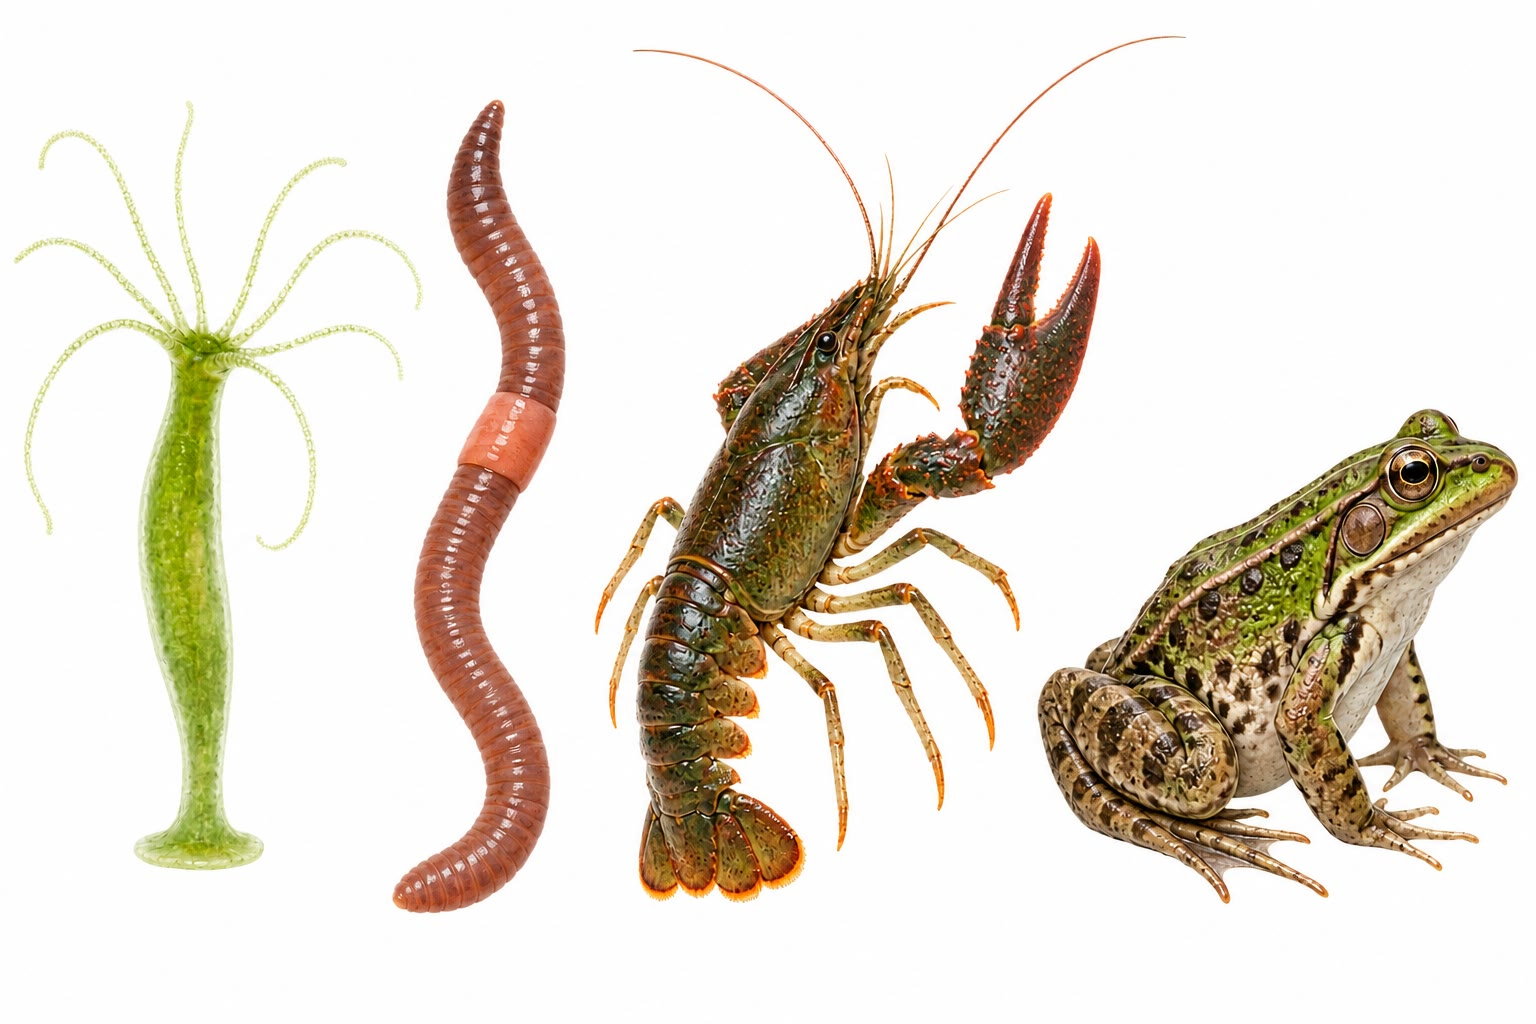
\includegraphics[width=0.78\linewidth]{images/book3/ai/b3-04-body-plans.jpg}

{\small 四种\omterm{def:b1:mammal-organization:bodyplan}{身体构型}。水螅（\omterm{def:b1:body-plans-tissues:symmetry}{辐射对称}、二\omterm{def:b1:body-plans-tissues:layers}{胚层}、无\omterm{def:b1:body-plans-tissues:layers}{体腔}），
蚯蚓（\omterm{def:b1:body-plans-tissues:symmetry}{两侧对称}、真\omterm{def:b1:body-plans-tissues:layers}{体腔}、\omterm{def:b1:body-plans-tissues:segments}{分节}、\omterm{def:b1:body-plans-tissues:segments}{流体静力骨骼}），
螯虾（\omterm{def:b1:body-plans-tissues:segments}{分节}且区段特化、关节式\omterm{def:b1:body-plans-tissues:segments}{外骨骼}），
以及青蛙（\omterm{def:b1:body-plans-tissues:proto}{后口动物}、骨质\omterm{def:b1:body-plans-tissues:segments}{内骨骼}）。}
\end{omfigure}

\begin{proposition}[四种构型比较]\label{prop:b1:body-plans-tissues:four}
\begin{center}
\small
\begin{tabular}{lllll}
\hline
 & 水螅 & 蚯蚓 & 螯虾 & 青蛙 \\
\hline
对称性 & 辐射 & 两侧 & 两侧 & 两侧 \\
\omterm{def:b1:body-plans-tissues:layers}{胚层}数 & 2 & 3 & 3 & 3 \\
\omterm{def:b1:body-plans-tissues:layers}{体腔} & 无 & 有 & 退化 & 有 \\
类群 &——& \omterm{def:b1:body-plans-tissues:proto}{原口动物} & \omterm{def:b1:body-plans-tissues:proto}{原口动物} & \omterm{def:b1:body-plans-tissues:proto}{后口动物} \\
体节 & 无 & 相似 & 特化 & 椎骨、肌块 \\
\omterm{def:b1:body-plans-tissues:segments}{骨骼} & 流体静力 & 流体静力 & \omterm{def:b1:body-plans-tissues:segments}{外骨骼} & \omterm{def:b1:body-plans-tissues:segments}{内骨骼} \\
肠道 & 单一开口 & 口到肛门 & 口到肛门 & 口到肛门 \\
循环 & 无 & 闭式 & 开式 & 闭式，有心脏 \\
神经系统 & 网状 & 腹神经索 & 腹神经索 & 背神经索 \\
\hline
\end{tabular}
\end{center}
这些构型并非梯子上的梯级：每一种都是完整而成功的
动物生存方式之一，螯虾与青蛙
互为同时代的类群，而非彼此的祖先。
\end{proposition}

\begin{example}[由身体构型推断动物]\label{ex:b1:body-plans-tissues:reading}
具有头部末端、贯通的肠道、由相似环节组成的身体，且无硬质
部件：有\omterm{def:b1:body-plans-tissues:layers}{体腔}的\omterm{def:b1:body-plans-tissues:proto}{原口动物}，靠\omterm{def:b1:body-plans-tissues:segments}{流体静力骨骼}运动，
每个体节的\omterm{def:b1:body-plans-tissues:layers}{体腔}液依次由环肌与纵肌加压——
即正在钻洞的蚯蚓。具有关节化\omterm{def:b1:flowering-plant-organization:tissues}{角质层}
和特化体节的动物，即节肢动物，其生长必须经过
蜕皮。\omterm{def:b1:body-plans-tissues:symmetry}{两侧对称}、\omterm{def:b1:body-plans-tissues:segments}{分节}的肌块环绕由椎骨构成的
背轴：脊椎动物，其\omterm{def:b1:body-plans-tissues:segments}{内骨骼}持续生长。
\end{example}

\section{四种组织类型}

\begin{definition}[组织]\label{def:b1:body-plans-tissues:tissue}
\emph{组织}\index{组织}是由结构和起源相似的细胞，
连同它们产生的细胞外物质，
共同组织起来以执行某一共同功能。动物组织分为四类，
即\omterm{def:b1:body-plans-tissues:epithelium}{上皮}组织、\omterm{def:b1:body-plans-tissues:connective}{结缔组织}、\omterm{def:b1:body-plans-tissues:muscle}{肌肉组织}和\omterm{def:b1:body-plans-tissues:nervous}{神经组织}。每个\omterm{def:b1:mammal-organization:organ}{器官}
都是其中至少两类组织的组合。
\end{definition}

\begin{definition}[上皮组织]\label{def:b1:body-plans-tissues:epithelium}
\emph{上皮}\index{上皮}是由紧密排列的细胞
构成的薄层，覆盖体表或衬于腔的内表面，附着于一层薄的
\omterm{def:b1:body-plans-tissues:connective}{细胞外基质}，即\emph{基膜}\index{基膜}。其
细胞是\emph{极性的}\index{细胞极性}：顶面朝向
外部或管腔，基面朝向基膜，两面所含的
蛋白质不同。细胞之间通过\emph{细胞
连接}\index{细胞连接}：靠近顶端的\emph{紧密连接}，
封闭细胞间隙，使任何物质都不能越过片层，
只能穿过细胞；\emph{黏着连接}和
\emph{桥粒}，二者机械性地把细胞牢固固定；\emph{缝隙
连接}，是允许离子和小分子由一个细胞
进入另一个细胞的通道。上皮依层数（单层、
复层）和细胞形状（扁平、立方、柱状）分类，
并包括腺体，即特化用于
分泌的上皮细胞。上皮的功能是覆盖、保护、吸收和分泌。
\end{definition}

\begin{omfigure}
\begin{tikzpicture}[font=\footnotesize, line cap=round]
  % three columnar cells
  \foreach \x in {0,1.6,3.2} {
    \draw[thick, fill=omDef!10] (\x,0) rectangle (\x+1.5,3.2);
    \fill[omDef!60] (\x+0.75,0.9) ellipse (0.32 and 0.42);
    % microvilli
    \foreach \m in {0.15,0.35,0.55,0.75,0.95,1.15,1.35} \draw[omDef!70!black, thick] (\x+\m,3.2) -- (\x+\m,3.5);
  }
  % junctions between cell 1-2 and 2-3
  \foreach \x in {1.55,3.15} {
    \draw[very thick, omThm] (\x-0.05,2.9) -- (\x+0.1,2.9);
    \draw[very thick, omProp] (\x-0.05,2.5) -- (\x+0.1,2.5);
    \draw[very thick, omProp] (\x-0.05,1.9) -- (\x+0.1,1.9);
    \draw[very thick, omExo] (\x-0.05,1.2) -- (\x+0.1,1.2);
  }
  % basal lamina
  \draw[very thick, gray!70] (-0.2,-0.05) -- (4.9,-0.05);
  \fill[pattern=north east lines, pattern color=gray!50] (-0.2,-0.6) rectangle (4.9,-0.1);
  % labels
  \node[anchor=south] at (2.4,3.55) {顶面：微绒毛，朝向管腔};
  \node[anchor=west, omThm] at (5.1,2.9) {紧密连接：封闭间隙};
  \node[anchor=west, omProp] at (5.1,2.5) {黏着连接：肌动蛋白环带};
  \node[anchor=west, omProp] at (5.1,1.9) {桥粒：机械铆钉};
  \node[anchor=west, omExo] at (5.1,1.2) {缝隙连接：细胞间通道};
  \node[anchor=west, gray!80!black] at (5.1,-0.05) {基膜};
  \node[anchor=west, gray!80!black] at (5.1,-0.45) {下方为结缔组织};
  \node[anchor=east] at (-0.3,0.9) {细胞核};
\end{tikzpicture}

{\small 单层柱状\omterm{def:b1:body-plans-tissues:epithelium}{上皮}，如肠道中所见。每个细胞
具有带微绒毛的顶面，以及位于\omterm{def:b1:body-plans-tissues:epithelium}{基膜}上的基面；
相邻细胞之间由紧密连接封闭，由黏着连接
和桥粒固定，并通过缝隙连接相通。}
\end{omfigure}

\begin{definition}[结缔组织]\label{def:b1:body-plans-tissues:connective}
\emph{结缔组织}\index{结缔组织}由散布的细胞
和它们分泌的大量\emph{细胞外基质}\index{细胞外基质}构成：蛋白质纤维——\emph{胶原蛋白}\index{胶原蛋白}
（抗拉强度高，占哺乳动物全部蛋白质的四分之一），
\emph{弹性蛋白}\index{弹性蛋白}（具回弹性）——嵌埋于富含水分的
多糖\emph{基质}中。依各成分比例可区分其类型：
疏松结缔\omterm{def:b1:body-plans-tissues:tissue}{组织}位于\omterm{def:b1:body-plans-tissues:epithelium}{上皮}下方及\omterm{def:b1:mammal-organization:organ}{器官}周围
（含成纤维细胞，纤维少而基质多）；致密结缔\omterm{def:b1:body-plans-tissues:tissue}{组织}
见于肌腱和韧带（胶原纤维平行排列）；脂肪\omterm{def:b1:body-plans-tissues:tissue}{组织}
（储存脂肪的细胞）；软骨（胶原与多糖构成的坚实凝胶，
无血管）；骨（胶原经磷酸钙矿化，
活细胞位于腔隙中，有血管）；血液，其基质为
\omterm{def:b1:mammal-organization:compartments}{血浆}。结缔\omterm{def:b1:body-plans-tissues:tissue}{组织}具有连接、支持、储存、运输和防御的功能。
\end{definition}

\begin{definition}[肌肉组织]\label{def:b1:body-plans-tissues:muscle}
\emph{肌肉组织}\index{肌肉组织}由细长的细胞构成，
细胞内充满收缩性蛋白丝（肌动蛋白和肌球蛋白）。共有
三类：\emph{\omterm{def:b1:body-plans-tissues:segments}{骨骼}肌}，由长的多核肌纤维构成，
具有横纹，附着于\omterm{def:b1:body-plans-tissues:segments}{骨骼}并受意识控制；
\emph{心肌}，由有分支的横纹细胞构成，细胞首尾借
连接相接，使搏动从一个细胞传给下一个细胞，并按自身
节律收缩；\emph{平滑肌}，由梭形、无横纹的细胞构成，位于
中空\omterm{def:b1:mammal-organization:organ}{器官}（肠道、血管、子宫）的管壁中，收缩缓慢且
不受意识控制。收缩的机制在
本科二年级分册中讨论。
\end{definition}

\begin{definition}[神经组织]\label{def:b1:body-plans-tissues:nervous}
\emph{神经组织}\index{神经组织}由
\emph{神经元}\index{神经元}，即具有胞体和长突起的细胞
（树突接收信号，轴突将信号传出），它们传导
电信号，并在突触处将信号传给其他细胞，并由
\emph{神经胶质细胞}\index{神经胶质细胞}构成，其数量是神经元的数倍，
起支持、绝缘和营养神经元的作用。神经\omterm{def:b1:body-plans-tissues:tissue}{组织}的功能是感知、整合
并发出指令。
\end{definition}

\begin{omfigure}
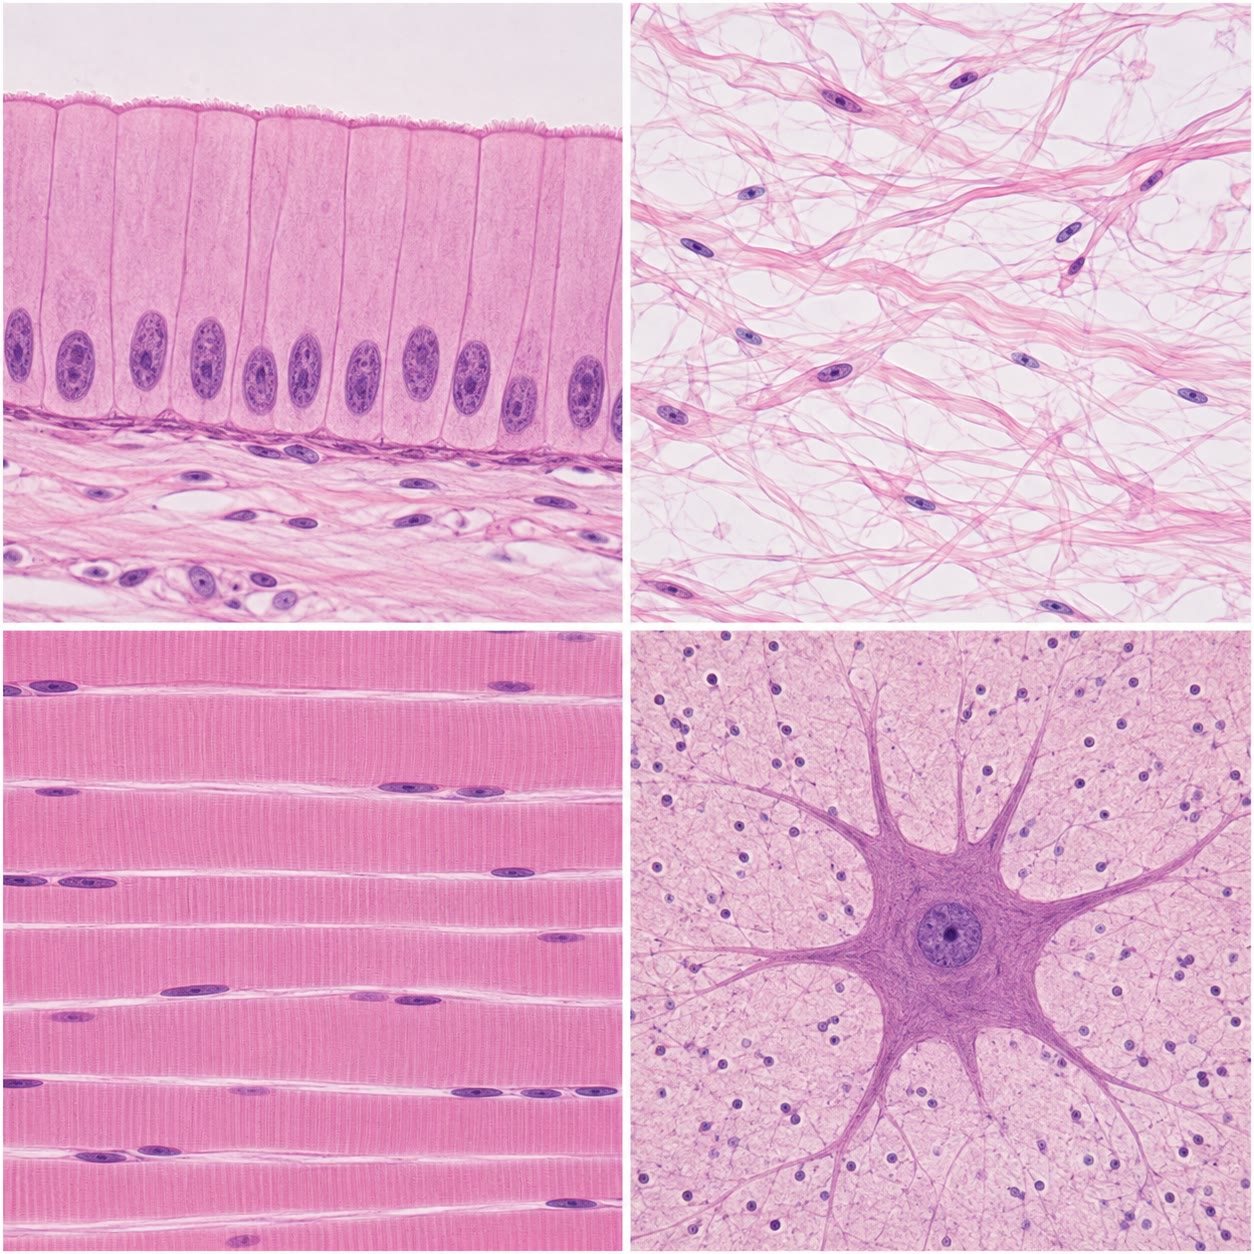
\includegraphics[width=0.6\linewidth]{images/book3/ai/b3-04-tissues.jpg}

{\small 显微镜下的四种\omterm{def:b1:body-plans-tissues:tissue}{组织}类型。左上：单层柱状\omterm{def:b1:body-plans-tissues:epithelium}{上皮}，
由一排高细胞构成。右上：疏松\omterm{def:b1:body-plans-tissues:connective}{结缔组织}，散布的细胞
位于波浪状的胶原纤维之间。左下：\omterm{def:b1:body-plans-tissues:segments}{骨骼}肌纤维，有横纹，
细胞核位于纤维边缘。
右下：\omterm{def:b1:body-plans-tissues:nervous}{神经元}与\omterm{def:b1:body-plans-tissues:nervous}{神经胶质细胞}。}
\end{omfigure}

\begin{example}[组织的来源]\label{ex:b1:body-plans-tissues:origin}
\omterm{def:b1:body-plans-tissues:epithelium}{上皮}分别来自三个\omterm{def:b1:body-plans-tissues:layers}{胚层}：皮肤来自\omterm{def:b1:body-plans-tissues:layers}{外胚层}，
肠道内衬来自\omterm{def:b1:body-plans-tissues:layers}{内胚层}，血管与\omterm{def:b1:body-plans-tissues:layers}{体腔}的内衬来自\omterm{def:b1:body-plans-tissues:layers}{中胚层}；
\omterm{def:b1:body-plans-tissues:connective}{结缔组织}、肌肉和血液来自\omterm{def:b1:body-plans-tissues:layers}{中胚层}；\omterm{def:b1:body-plans-tissues:nervous}{神经组织}来自\omterm{def:b1:body-plans-tissues:layers}{外胚层}。
蛙的皮肤是覆于\omterm{def:b1:body-plans-tissues:layers}{中胚层}\omterm{def:b1:body-plans-tissues:connective}{结缔组织}之上的\omterm{def:b1:body-plans-tissues:layers}{外胚层}\omterm{def:b1:body-plans-tissues:epithelium}{上皮}；
其肠道是包裹在\omterm{def:b1:body-plans-tissues:layers}{中胚层}肌肉中的\omterm{def:b1:body-plans-tissues:layers}{内胚层}\omterm{def:b1:body-plans-tissues:epithelium}{上皮}；
其脑则是向内折叠的\omterm{def:b1:body-plans-tissues:layers}{外胚层}。
\end{example}

\section{从组织到器官：消化管的管壁}

\begin{proposition}[消化管壁的四层结构]\label{prop:b1:body-plans-tissues:gutwall}
\index{消化管壁}
从管腔向外，脊椎动物消化管的管壁由
四层同心层构成，每一层都由若干\omterm{def:b1:body-plans-tissues:tissue}{组织}组合而成：
\emph{黏膜}（\omterm{def:b1:body-plans-tissues:epithelium}{上皮}——兼具吸收与分泌功能——位于疏松\omterm{def:b1:body-plans-tissues:connective}{结缔组织}之上，
\omterm{def:b1:body-plans-tissues:connective}{结缔组织}中有血管和淋巴管，其下有一薄层平滑肌）；
\emph{黏膜下层}（致密\omterm{def:b1:body-plans-tissues:connective}{结缔组织}，
含较粗的血管和神经网络）；\emph{肌层}（两层
平滑肌，内环行、外纵行，二者之间
有神经网络，负责混合与推进运动）；
以及\emph{浆膜}（一薄层\omterm{def:b1:body-plans-tissues:connective}{结缔组织}，
外覆\omterm{def:b1:body-plans-tissues:layers}{体腔}\omterm{def:b1:body-plans-tissues:epithelium}{上皮}）。从食管到直肠，四层结构
始终相同，变化的是黏膜：在小肠中折叠成绒毛，
在胃中则为腺性。
\end{proposition}

\begin{omfigure}
\begin{tikzpicture}
  \node[anchor=south west, inner sep=0] (img) at (0,0)
    {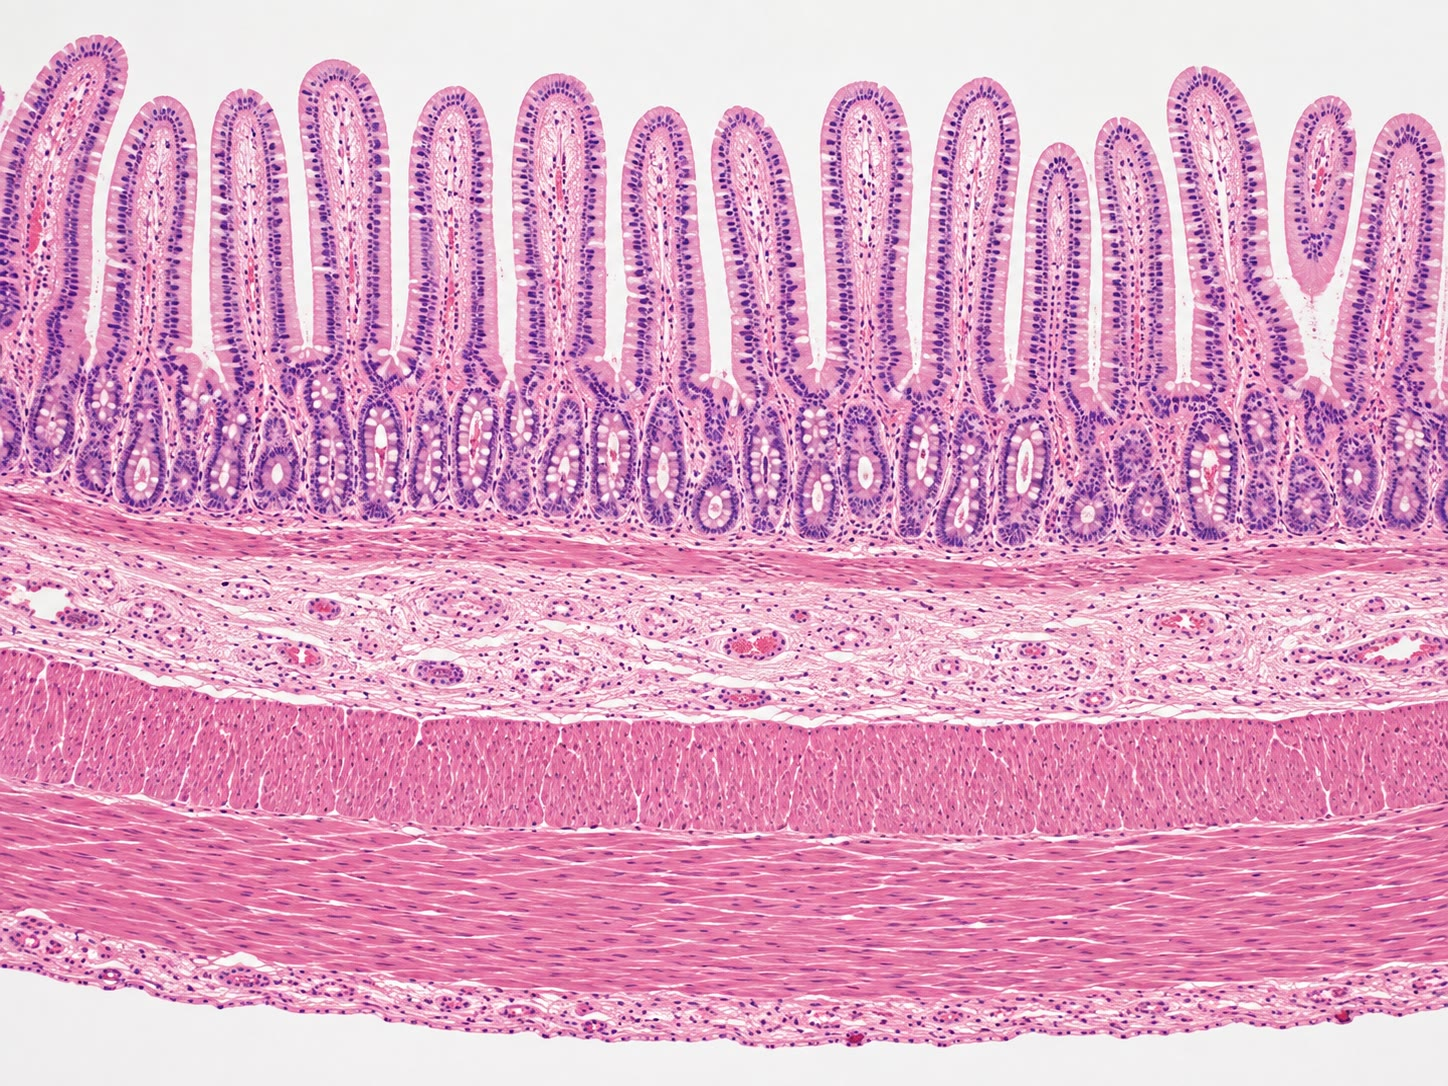
\includegraphics[width=0.53\linewidth]{images/book3/ai/fig-gut-wall-histology.jpg}};
  \begin{scope}[x={(img.south east)}, y={(img.north west)},
      every node/.style={font=\small}]
    \draw[omDef, thick] (0.50,0.985) -- (0.50,1.08) node[above] {管腔};
    \draw[omDef, thick] (0.30,0.82) -- (-0.03,0.86) node[left, align=right] {绒毛：上皮 \\ 位于结缔组织之上};
    \draw[omDef, thick] (0.40,0.58) -- (-0.03,0.56) node[left] {腺体（隐窝）};
    \draw[omDef, thick] (0.70,0.505) -- (1.03,0.56) node[right] {黏膜肌层};
    \draw[omDef, thick] (0.70,0.42) -- (1.03,0.42) node[right] {黏膜下层};
    \draw[omDef, thick] (0.70,0.24) -- (1.03,0.26) node[right, align=left] {肌层：\\ 环行、纵行};
    \draw[omDef, thick] (0.70,0.06) -- (1.03,0.06) node[right] {浆膜};
  \end{scope}
\end{tikzpicture}

{\small 小肠管壁的横切面。黏膜的绒毛伸入管腔；
其下依次为腺体、一薄层肌肉、
黏膜下层、两层肌层
和浆膜。四层结构，四类\omterm{def:b1:body-plans-tissues:tissue}{组织}，一个\omterm{def:b1:mammal-organization:organ}{器官}。}
\end{omfigure}

\begin{method}[组织切片的读图方法]\label{met:b1:body-plans-tissues:histology}
\begin{enumerate}
  \item 找到游离面或管腔：内衬其上的\omterm{def:b1:body-plans-tissues:epithelium}{上皮}
        即为第一层。数清其细胞核的层数（单层
        或复层），并注意细胞的形状。
  \item 在\omterm{def:b1:body-plans-tissues:epithelium}{上皮}之下寻找浅色的纤维区，
        其中散布细胞核和血管：即\omterm{def:b1:body-plans-tissues:connective}{结缔组织}。
  \item 肌肉表现为细长细胞构成的密集束：
        \omterm{def:b1:body-plans-tissues:segments}{骨骼}肌有横纹，细胞核位于边缘；心肌有横纹且有分支；
        平滑肌无横纹，细胞核位于中央。注意
        纤维相对于切面的方向。
  \item \omterm{def:b1:mammal-organization:organ}{器官}管壁中的\omterm{def:b1:body-plans-tissues:nervous}{神经组织}表现为位于肌层之间的
        大而浅色的\omterm{def:b1:body-plans-tissues:nervous}{神经元}胞体团。
  \item 根据各层的排列顺序和
        黏膜的特化结构（绒毛、腺体、角质）判断\omterm{def:b1:mammal-organization:organ}{器官}名称。
\end{enumerate}
\end{method}

\begin{example}[绒毛作为交换面]\label{ex:b1:body-plans-tissues:villus}
人类小肠的一个绒毛是一个高\qty{0.6}{mm}、
宽\qty{0.15}{mm}的指状突起，表面覆盖一层柱状细胞，
每个细胞的顶端表面约有\qty{1500}{}个微绒毛。绒毛使肠管表面积增加约七倍，
微绒毛再使其增加约二十倍：
原本\qty{0.6}{m^2}的平直管道变为数十平方米的吸收性\omterm{def:b1:body-plans-tissues:epithelium}{上皮}，
厚度仅一个细胞，每个细胞距其绒毛\omterm{def:b1:body-plans-tissues:connective}{结缔组织}核心中的
毛细血管和淋巴管仅数微米（见\cref{ch:b1:digestion-absorption}）。
\omterm{def:b1:body-plans-tissues:epithelium}{上皮}每四天由其基部的腺体更新一次：
\omterm{def:b1:body-plans-tissues:epithelium}{上皮}层、其连接和极性
都在持续重建。
\end{example}

\begin{remark}[两种模式生物的组织]\label{rem:b1:body-plans-tissues:plants}
\cref{ch:b1:flowering-plant-organization}中植物的三个\omterm{def:b1:body-plans-tissues:tissue}{组织}系统，
与这里的\omterm{def:b1:body-plans-tissues:tissue}{组织}并无严格的对应关系。植物的\omterm{def:b1:flowering-plant-organization:tissues}{表皮}在功能上是一种\omterm{def:b1:body-plans-tissues:epithelium}{上皮}，
但其细胞靠细胞壁相连，而非靠\omterm{def:b1:body-plans-tissues:epithelium}{细胞连接}；其\omterm{def:b1:flowering-plant-organization:tissues}{基本组织}同时承担
储存、支持与光合作用；植物既无肌肉，也无神经。
动物的四类\omterm{def:b1:body-plans-tissues:tissue}{组织}是能够运动和感知的身体所用的“工具箱”，
而植物的三类\omterm{def:b1:body-plans-tissues:tissue}{组织}则属于能够生长的身体。
\end{remark}

\section{练习}

\begin{exercise}[$\star$]\label{exo:b1:body-plans-tissues:1}
定义\omterm{def:b1:body-plans-tissues:symmetry}{辐射对称}和\omterm{def:b1:body-plans-tissues:symmetry}{两侧对称}，并各举一种动物为例。
哪一种与\omterm{def:b1:mammal-organization:bodyplan}{头部集中化}相伴？为什么？
\end{exercise}

\begin{exercise}[$\star$]\label{exo:b1:body-plans-tissues:2}
说出三个\omterm{def:b1:body-plans-tissues:layers}{胚层}，并各举出一种由其衍生的\omterm{def:b1:body-plans-tissues:tissue}{组织}。
\end{exercise}

\begin{exercise}[$\star$]\label{exo:b1:body-plans-tissues:3}
列出四种\omterm{def:b1:body-plans-tissues:tissue}{组织}类型，并说明每种的定义性特征与
各自的一项功能。
\end{exercise}

\begin{exercise}[$\star$]\label{exo:b1:body-plans-tissues:4}
根据\omterm{def:b1:body-plans-tissues:epithelium}{上皮}图，说出从顶端到基部的四种连接
及各自的作用。
\end{exercise}

\begin{exercise}[$\star\star$]\label{exo:b1:body-plans-tissues:5}
某动物具有三个\omterm{def:b1:body-plans-tissues:layers}{胚层}、一个由\omterm{def:b1:body-plans-tissues:layers}{中胚层}衬里的\omterm{def:b1:body-plans-tissues:layers}{体腔}、
贯通式消化道、相似的体节且无硬体部分。逐一说明其\omterm{def:b1:mammal-organization:bodyplan}{身体构型}特征，
并指出一个与之相符的类群。
\end{exercise}

\begin{exercise}[$\star\star$]\label{exo:b1:body-plans-tissues:6}
解释蚯蚓如何以\omterm{def:b1:body-plans-tissues:layers}{体腔}作为\omterm{def:b1:body-plans-tissues:segments}{骨骼}进行运动，
并结合每一体节的两层肌肉加以说明。
\end{exercise}

\begin{exercise}[$\star\star$]\label{exo:b1:body-plans-tissues:7}
比较小龙虾的\omterm{def:b1:body-plans-tissues:segments}{外骨骼}与青蛙的\omterm{def:b1:body-plans-tissues:segments}{内骨骼}，
从生长、保护、肌肉附着，以及各自施加的体型限制等方面
进行比较。
\end{exercise}

\begin{exercise}[$\star\star$]\label{exo:b1:body-plans-tissues:8}
\omterm{def:b1:body-plans-tissues:epithelium}{上皮}要成为受\omterm{def:b1:organism-environment:organism}{生物体}控制的交换表面，
为何需要紧密连接？若无紧密连接，
肠道吸收会发生什么变化？
\end{exercise}

\begin{exercise}[$\star\star$]\label{exo:b1:body-plans-tissues:9}
某切片自管腔向外依次为：带绒毛的单层柱状\omterm{def:b1:body-plans-tissues:epithelium}{上皮}、
疏松\omterm{def:b1:body-plans-tissues:connective}{结缔组织}、薄层肌肉、致密\omterm{def:b1:body-plans-tissues:connective}{结缔组织}、两层厚肌肉、
以及薄的外层。指出该\omterm{def:b1:mammal-organization:organ}{器官}及其每一层
的名称。
\end{exercise}

\begin{exercise}[$\star\star\star$]\label{exo:b1:body-plans-tissues:10}
软骨无血管，骨则血管丰富。试将此与二者各自的营养方式、
愈合速度相联系，
并说明二者在体内的分布部位。
\end{exercise}

\begin{exercise}[$\star\star\star$]\label{exo:b1:body-plans-tissues:11}
某药物阻断肠\omterm{def:b1:body-plans-tissues:epithelium}{上皮}中紧密连接的形成。
试依据\omterm{def:b1:body-plans-tissues:epithelium}{上皮}的性质，预测该药物对吸收、
\omterm{def:b1:organism-environment:milieu}{内环境}组成以及感染的影响，
并加以说明。
\end{exercise}

\begin{exercise}[$\star\star\star$]\label{exo:b1:body-plans-tissues:12}
“\omterm{def:b1:mammal-organization:bodyplan}{身体构型}是一组约束，而非设计。”在一段文字中，结合
节肢动物的蜕皮、昆虫的体型、脊椎动物的体节，
以及本章表格的含义加以讨论。
\end{exercise}

\section{问题：小肠的管壁}

\begin{problem}[{周末问题——人体小肠的组织学切片系列，
从肠管一直读到微绒毛：层次、
绒毛、细胞、连接与更新，最终落在单个
绒毛的吸收表面}]
\label{pb:b1:body-plans-tissues:1}
人体小肠是一根长 \qty{6}{m}、内径 \qty{3}{cm} 的管道。
管壁的环形皱襞使
光滑管的表面积增至三倍。其黏膜上每平方毫米
褶皱表面带有 \qty{25}{} 个绒毛，每个绒毛为高 \qty{0.6}{mm}、
直径 \qty{0.15}{mm} 的圆柱体。绒毛表面覆盖着柱状细胞，其顶端面为
边长 \qty{5}{\micro m} 的正方形；每个顶端面带有
\qty{1500}{} 根微绒毛，每根为长 \qty{1}{\micro m}、
直径 \qty{0.1}{\micro m} 的圆柱体。\omterm{def:b1:body-plans-tissues:epithelium}{上皮}每隔
\qty{4}{} 天更新一次。

\medskip
\noindent\textbf{第一部分——各层。}
在显微镜下观察一张横切片。
\begin{enumerate}
  \item 自管腔向外列出管壁的四层结构，以及
        每层中的\omterm{def:b1:body-plans-tissues:tissue}{组织}类型。
  \item 切片中可见绒毛，该切片取自消化管的哪一段？
        若是胃的切片，将会看到什么？
  \item 在肌层的两层肌肉之间，分布着成团的
        大而色淡的细胞。它们是什么？它们调控什么？
  \item 解释为何两层肌肉的走向
        相互垂直。
\end{enumerate}

\medskip
\noindent\textbf{第二部分——表面积。}
\begin{enumerate}[resume]
  \item 计算光滑管的内表面积。
  \item 计算加上环形皱襞后的表面积。
  \item 计算单个绒毛的侧面积（视为圆柱，忽略
        顶端）。
  \item 计算每平方毫米褶皱黏膜上绒毛的表面积，
        以及绒毛使表面积增大的倍数。
  \item 计算加上绒毛后的表面积。
  \item 计算单根微绒毛的侧面积，以及
        一个细胞上 \qty{1500}{} 根微绒毛的侧面积。
  \item 计算微绒毛使单个细胞顶端表面积增大的
        倍数。
  \item 计算小肠的总吸收表面积。
\end{enumerate}

\medskip
\noindent\textbf{第三部分——细胞。}
\begin{enumerate}[resume]
  \item 计算覆盖单个绒毛的\omterm{def:b1:body-plans-tissues:epithelium}{上皮}细胞数。
  \item 计算小肠中的绒毛数，以及覆盖它们的
        \omterm{def:b1:body-plans-tissues:epithelium}{上皮}细胞数。
  \item \omterm{def:b1:body-plans-tissues:epithelium}{上皮}每隔 \qty{4}{} 天更新一次。每天有多少细胞
        脱落进入管腔？每秒又是多少？
  \item 替换细胞产生于何处？
        这说明分裂中的细胞
        相对于吸收细胞的位置如何？
  \item 一个\omterm{def:b1:body-plans-tissues:epithelium}{上皮}细胞高 \qty{25}{\micro m}。计算
        小肠\omterm{def:b1:body-plans-tissues:epithelium}{上皮}的体积及其质量
        （密度 \qty{1.05}{g/cm^3}）。
\end{enumerate}

\medskip
\noindent\textbf{第四部分——连接、基质与绒毛。}
\begin{enumerate}[resume]
  \item 每个细胞通过环绕其顶端的紧密连接与相邻细胞密封。
        计算每个细胞的紧密连接长度，
        以及小肠中紧密连接的总长度。
  \item 解释管腔中的物质为何只有穿过
        两层细胞膜才能进入血液。
  \item 绒毛的核心是疏松\omterm{def:b1:body-plans-tissues:connective}{结缔组织}，内含毛细血管网
        和位于中央的淋巴管。指出其中所含的
        两类细胞外纤维及分泌它们的
        细胞。
  \item 指出\omterm{def:b1:body-plans-tissues:epithelium}{上皮}及
        绒毛核心各自的起源\omterm{def:b1:body-plans-tissues:layers}{胚层}。
  \item 绒毛中还含有一束平滑肌，使其
        有节律地收缩。试推测其功能。
  \item 某疾病使绒毛变平（表面积回到
        褶皱管的表面积）。吸收表面积降低了多少倍，
        造成的后果是什么？
  \item 计算单个绒毛连同其微绒毛的吸收表面积，
        以平方毫米为单位。
  \item 写出结果：单个绒毛的吸收表面积，
        以及小肠中的绒毛数。
\end{enumerate}
\end{problem}
